
\documentclass{article}


% The file ijcai11.sty is the style file for IJCAI-11 (same as ijcai07.sty).
\usepackage{ijcai11,times,graphicx,amsmath,float,multirow,bbm,amssymb}


\title{Gesture Alignment Using Hidden Markov Models}
\author{
Andrew Hershberger
\quad Salman Ahmad \\
\{andrew.hershberger, saahmad\}@stanford.edu
\\\\
Stanford University\\
CS228: Probabilistic Graphical Methods --- Winter 2011\\
}

\begin{document}

\maketitle

\begin{abstract}

Gesture recognition gaining interest in many domains. A common issue when
learning from multiple training gestures is accounting for noise and different
durations and speeds. This paper presents an algorithm that uses Hidden Markov
Models to align training gestures and learn the hidden canonical gesture that
they represent. The algorithm was used to align motion capture data from an
Xbox Kinect. This paper present initial results along with a discussion of
current limitations and paths for future work.

\end{abstract}

\section{Introduction}

Gesture recognition is becoming increasingly important in many fields from
gaming to user interface design. Since it is difficult to manually encode
gestures declaratively, there is a lot of interest in applying learning
techniques to train a classifier that can recognize gestures from motion
capture data.

A common problem with this approach is that the training examples are often
different durations and different speeds. This paper provides an algorithm
that aligns gestures based on the important actions that take place - e.g. the
start of a wave or the midpoints in a jump. Additionally, the algorithm
learns a canonical representation of the gesture that can be used for
classification of new data.

\begin{figure}
\begin{centering}
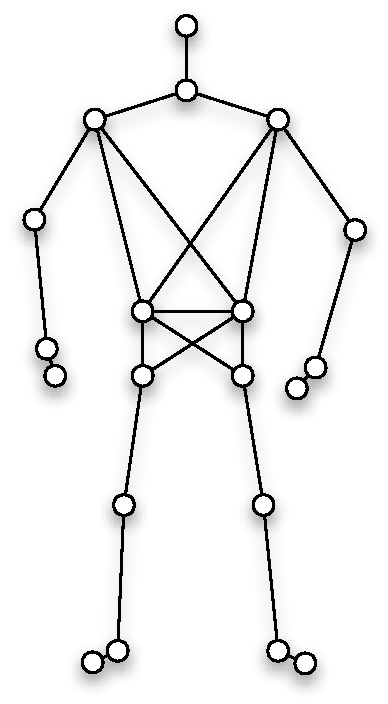
\includegraphics[width=0.4\columnwidth]{figures/control_points.pdf}

\caption{The location twenty control points that are tracked by the gesture
alignment algorithm.\label{figure:control_points}}

\end{centering}
\end{figure}

The algorithm was evaluated using motion capture information from an Xbox
Kinect. The raw RGBZ output was converted to \emph{(x,y,z)} positions of 20
different control points on the human body as shown in Figure
\ref{figure:control_points}. An alignment hidden markov model was then used to
align the different gestures.

The rest of this paper presents related work in this area, the graphical model
used to encode the independencies of the data, a discussion of the algorithm,
results, an analysis of current limitations, and logical areas of future work.


\section{Related Work}

Koller and Friedman \cite{Koller2009} provide an overview and analysis of
different approaches to solving sequence labeling problems like gesture
recognition. The hidden Markov model (HMM), a generative model, presents
the challenge of modeling a distribution over the observed variables. By
contrast, the maximum entropy Markov model (MEMM) and conditional random
field (CRF) are discriminative approaches in which only the conditional
distribution over the class labels must be modeled, thus avoiding the need to
model the distribution over the observed variables directly. On the other hand,
generative models may allow learning with less training data than would be
required in the discriminative case.

In one gesture recognition project, Wang et al.\ \cite{Wang2006} employed a
CRF variant called a hidden conditional random field (HCRF). Their approach,
however, did not address the issue of dealing with varying length gestures or
gestures that are compressed or expanded in time during various phases.

In a related study, Coates et al.\ \cite{Coates2008} addressed the problem of
learning an ideal pattern from multiple non-ideal demonstrations. They applied
an iterative expectation maximization (EM) algorithm for aligning multiple input
sequences while simultaneously learning the ideal target sequence. Their
approach interleaved iterations of a Kalman smoother and dynamic time warping.
The Kalman smoother \cite{Muphy2002} was used to determine the means and
covariance matrices of the hidden target sequence. The dynamic time warping
algorithm \cite{Listgarten2005} then determined the highest-likelihood mapping
of the observed sequences onto the ideal. Eventually this iterative process
converged producing tremendous results.

\section{Graphical Model}

\begin{figure}
\begin{centering}
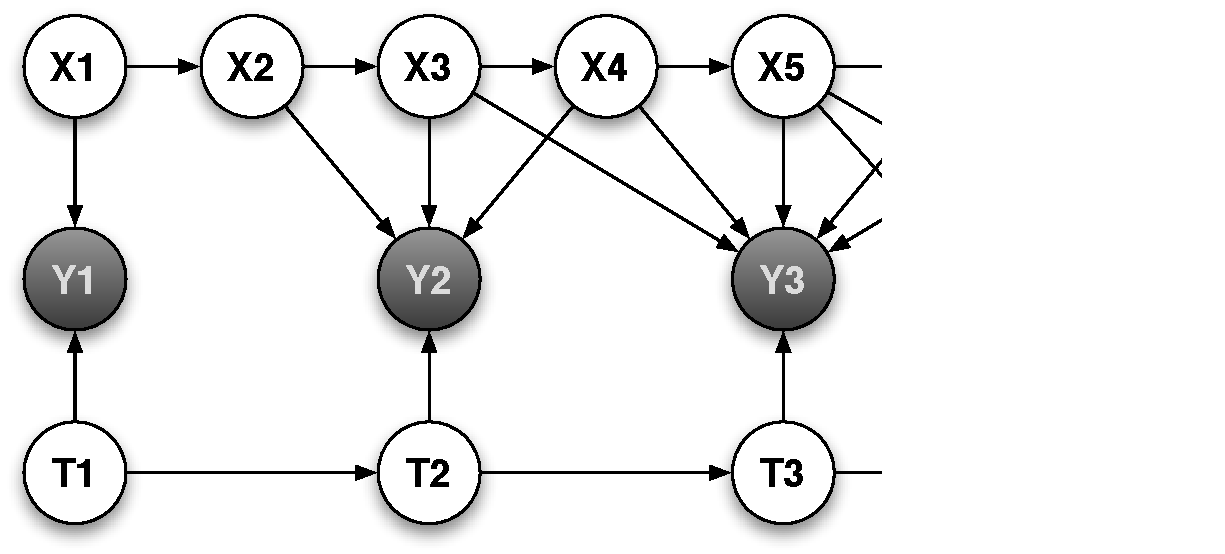
\includegraphics[width=0.65\columnwidth]{figures/model_tau_unobserved.pdf}

\caption{The graphical model using for gesture alignment. $\mathbf{Z}$
represents the hidden, ``canonical'' gesture. $\mathbf{Y}$ represents the
observed gesture from the training set. $\mathbf{T}$ represents an indexed
mapping between the observed gesture to the canonical gesture. The dark nodes
are observed. \label{figure:model_tau_unobserved}}

\end{centering}
\end{figure}


The algorithm uses an alignment HMM to align observed gestures. The graphical
representation of the model is shown in Figure \ref{figure:model_tau_unobserved}
and is similar to the model proposed by \cite{Coates2008}. The model involves
three important variables. $\mathbf{Z}$ is the ideal, canonical gesture. It is a
hidden variables that is learned. $\mathbf{Y}$ is one of the observed gestures
that is used for learning. $\mathbf{T}$ is a mapping variables that indicates
which frame in $\mathbf{Y}$ is matched to a frame in $\mathbf{Z}$.

The model tries to match the $\mathbf{Y}$ to $\mathbf{Z}$ by searching to see
which frames in the two gestures form the best match. Frames are matched using a
dynamic time warping and is described in greater detail in the algorithm section
below. In essence, the dynamic time warping maintains the temporal dependencies
between the two gestures by only search over a fixed number of frames - a so
called \emph{step size}. In figure \ref{figure:model_tau_unobserved} the step
size is 3; however, in practice we found that larger step sizes close to 25
produced the best results for our datasets.

Once two frames have been matched, the graphical model imposes a restriction
that prevents frames to be matched out of order as described. For example, if
frame 20 of $\mathbf{Y}$ is matched to frame 30 in $\mathbf{Z}$, then the model
would prevent any frame greater than 20 in $\mathbf{Y}$ to be matched to any
frame less than 30 in $\mathbf{Z}$.

As said before, the model encodes two sets of hidden variables, the mapping
$\mathbf{T}$ and the canonical gestures $\mathbf{Z}$. The algorithm uses an
Estimation Maximization approach to solve for both these variables. Once
$\mathbf{T}$ is known, the algorithm attempts to learn $\mathbf{Z}$ from
$\mathbf{Y}$. At this point the graphical model has transformed to look like
Figure \ref{figure:model_tau_observed}.

As is evident from Figure \ref{figure:model_tau_unobserved}, the canonical
gesture will be much longer than the observed training gestures. This is done to
account for the gestures of different lengths. In practice we found that a good
length for $\mathbf{Z}$ is approximately twice as long as the average length of
the training gestures as shown below:

\[
	|Z| = \frac{2 \cdot \sum_{i}{Y_i}}{|\mathbf{Y}|}
\]

\begin{figure}
\begin{centering}
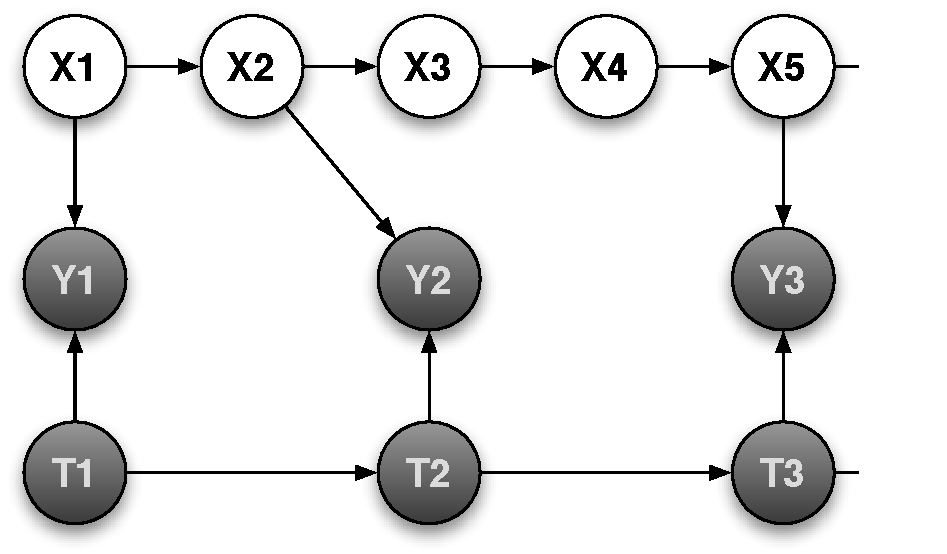
\includegraphics[width=0.63\columnwidth]{figures/model_tau_observed.pdf}

\caption{An example graphical model once $\mathbf{T}$ has been learned. In this
case, the second and third frames from the observed gesture maps to the second
and fifth frame of the canonical gesture. The dark nodes are observed.
\label{figure:model_tau_observed}}

\end{centering}
\end{figure}


\section{Algorithm}

ANDREW:

We decided to focus on the alignment HMM subproblem of the larger gesture
recognition problem. This is a particularly important issue in cases where it is
important to allow gestures of different speeds or of varying speed to be
recognized by the system.

We chose to follow the general approach outlined by Coates et al.\
\cite{Coates2008} where smoothing EM steps were interleaved with dynamic time
warping EM steps. We also did several things differently. First, we used a local
regression weighted linear least squares smoother. We turned to this approach
because the Kalman smoother requires a notion of a dynamics model that is used
to calculate the next state given the current state and noise.

In our case, generating such a model is infeasible because of the large
variation in the way different people perform the same gesture. Secondly, we
also did not incorporate prior knowledge about the ideal gesture. As discussed
later, such information is a key area for future work to explore what kinds of
prior knowledge can be incorporated to improve performance.

Optimizing the algorithm when calculating q(:,:), tau;

no prior knowledge of optimal trajectory

not using a bias function

Tried different allowed step sizes for d

\section{Results}

We ran our algorithm on the data output from an Xbox Kinect. The Kinect outputs
RGBZ images which are analyzed and broken into 20 control points with
\emph{(x,y,z)} information.

Our training corpus consisted of several different types of gestures including:
clap, flick left, flick right, high kick, low kick, jump, punch, throw, and
wave. 



\begin{figure}
\begin{centering}

\begin{centering}
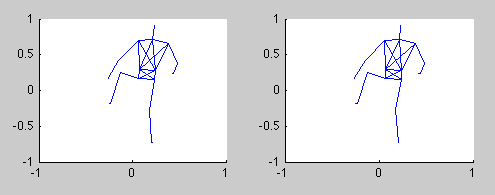
\includegraphics[width=\columnwidth]{figures/kick_aligned.png}	
\end{centering}
\begin{centering}
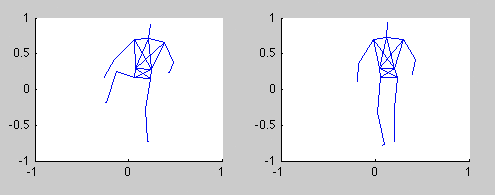
\includegraphics[width=\columnwidth]{figures/kick_unaligned.png}	
\end{centering}

\vspace{-0.2in}

\caption{Motion capture data of a person performing a kick. Top:
 Data that has
been aligned with our algorithm. Bottom: The Original, unaligned data. Both
images were taken at the same time offset. \label{figure:kick}}

\end{centering}
\end{figure}


The algorithm worked well in certain cases. For example, figure
\ref{figure:kick} shows a successful case in which a kick was aligned correctly.


Unfortunately, the algorithm has several short comings as well. In many cases,
the learned canonical gesture is very choppy and noisy. Furthermore, there are
many cases in which the aligned gestures violate physical properties of the
world. See figure \ref{figure:jump} as an example. A more detailed discussion of
current limitations and avenues for future work are provided in the next
section.




\section{Discussion and Future Work}

ANDREW:

Why didn't it work very well? Smoothing made things worse.

Use different smoothing

Add prior knowledge of optimal trajectory: can incorporate effects of gravity
- don't want things to hang in mid air.

Application to classification problem

Add more data (training data)

Add features to detect particular aspects of gestures.

Detect orientation differences



\section{Conclusion}


\begin{figure}
\begin{centering}
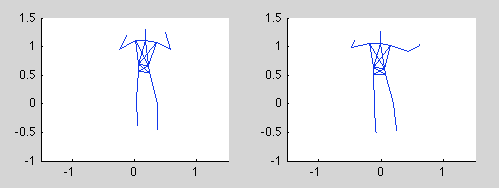
\includegraphics[width=\columnwidth]{figures/jump.png}

\caption{A failure case of our implementation. The algorithm does not have
domain specific information about the dynamics of the real world, for example,
gravity. The above data was taken from a person jumping. To align the data,
the algorithm ``freezes'' the person in mid-air when this is obviously
physically impossible. \label{figure:jump}}

\end{centering}
\end{figure}

This paper presents a method to perform gesture alignment using a Hidden
Markov Model. The algorithm was shown to be able to align certain gestures and
learn a canonical gesture. The method was applied to motion capture data that
was extracted from RGBZ images taken from an Xbox Kinect.

While the findings were some what promising it failed to work on a diverse set
of gestures. There are obvious areas for future work. First, the model should
incorporate our prior knowledge of the ideal gesture. For example, it would
certainly help to encode that during a kick, one of the legs will be
accelerating while the rest of the body stays still. Second, the algorithm
should incorporate a dynamics model of the real world. This will allow the
method to better deal with physical phenomenons like gravity.





\bibliographystyle{named}
\bibliography{CS228}

\end{document}
